\documentclass[tikz,border=2pt]{standalone}
\usepackage{amsmath}
\usetikzlibrary{shapes.geometric}
\definecolor{lvlone}{RGB}{31,119,180}
\definecolor{lvltwo}{RGB}{214,39,40}
\begin{document}
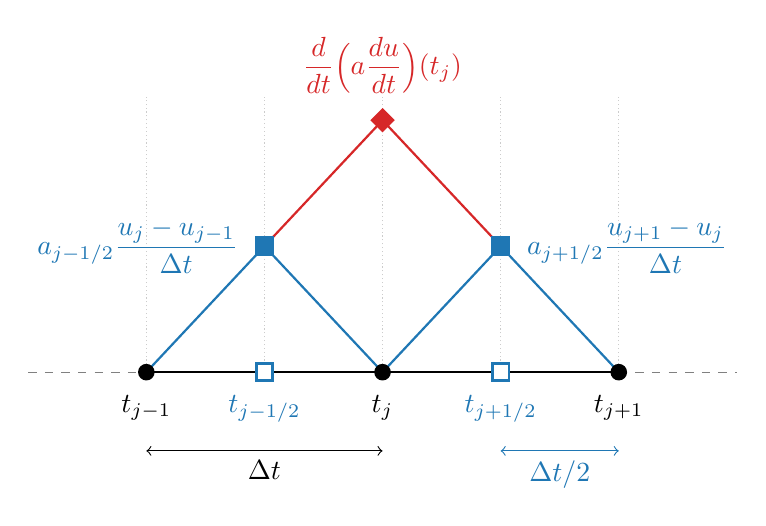
\begin{tikzpicture}[scale=1.0,
    gridpt/.style={circle, fill=black, inner sep=0pt, minimum size=6pt},
    stagpt/.style={rectangle, draw=lvlone, fill=white, line width=1pt, inner sep=0pt, minimum size=6pt},
    onept/.style={rectangle, fill=lvlone, inner sep=0pt, minimum size=7pt},
    twopt/.style={diamond, fill=lvltwo, inner sep=0pt, minimum size=9pt},
    ]
    \def\dt{3}
    \def\yone{1.6}
    \def\ytwo{3.2}
    % vertical guides
    \foreach \x in {-1,-0.5,0,0.5,1} {
        \draw[gray!40, densely dotted] (\x*\dt,0) -- (\x*\dt,\ytwo+0.3);
    }
    % grid line
    \draw[dashed, gray] (-1.5*\dt,0) -- (-1*\dt,0);
    \draw[dashed, gray] (1*\dt,0) -- (1.5*\dt,0);
    \draw[thick] (-1*\dt,0) -- (1*\dt,0);

    % level 1 connections: u at grid points -> (a u') at midpoints
    \foreach \m/\l/\r in {-0.5/-1/0, 0.5/0/1} {
        \draw[lvlone, thick] (\l*\dt,0) -- (\m*\dt,\yone);
        \draw[lvlone, thick] (\r*\dt,0) -- (\m*\dt,\yone);
    }
    % level 2 connections: midpoints -> t_j
    \draw[lvltwo, thick] (-0.5*\dt,\yone) -- (0,\ytwo);
    \draw[lvltwo, thick] (0.5*\dt,\yone) -- (0,\ytwo);

    % grid points (u values)
    \foreach \x/\lab in {-1/{j-1}, 0/{j}, 1/{j+1}} {
        \node[gridpt] at (\x*\dt,0) {};
        \node[below=5pt] at (\x*\dt,0) {$t_{\lab}$};
    }
    % staggered points for a
    \foreach \x/\lab in {-0.5/{j-1/2}, 0.5/{j+1/2}} {
        \node[stagpt] at (\x*\dt,0) {};
        \node[below=5pt, lvlone] at (\x*\dt,0) {$t_{\lab}$};
    }

    % level 1 points
    \node[onept] at (-0.5*\dt,\yone) {};
    \node[onept] at (0.5*\dt,\yone) {};
    \node[left=6pt, lvlone] at (-0.5*\dt,\yone)
        {$a_{j-1/2}\dfrac{u_j - u_{j-1}}{\Delta t}$};
    \node[right=6pt, lvlone] at (0.5*\dt,\yone)
        {$a_{j+1/2}\dfrac{u_{j+1} - u_j}{\Delta t}$};

    % level 2 point
    \node[twopt] at (0,\ytwo) {};
    \node[above=6pt, lvltwo] at (0,\ytwo)
        {$\dfrac{d}{dt}\Big(a\dfrac{du}{dt}\Big)(t_j)$};

    % spacing
    \draw[<->] (-1*\dt,-1.0) -- node[below] {$\Delta t$} (0,-1.0);
    \draw[<->, lvlone] (0.5*\dt,-1.0) -- node[below] {$\Delta t/2$} (1*\dt,-1.0);
\end{tikzpicture}
\end{document}
